\documentclass[aspectratio=169]{beamer}
\usepackage{graphicx}
\usepackage{xcolor}
\usepackage{tikz}

\definecolor{mainblue}{RGB}{0, 51, 102}
\definecolor{accentblue}{RGB}{0, 102, 204}

\usetheme{default}
\usecolortheme{whale}
\setbeamercolor{structure}{fg=mainblue}
\setbeamercolor{title}{fg=white}
\setbeamercolor{frametitle}{fg=mainblue}
\setbeamercolor{normal text}{fg=black}
\setbeamercolor{background canvas}{bg=white}
\setbeamercolor{block title}{bg=mainblue, fg=white}

\title{Student Dropout Prediction: A Machine Learning Analysis}
\subtitle{DSAA2011(L01) Course Project - HKUST(GZ) 2026 Spring}
\author{Hao LUO, Congren HANG, Xingjian LI, Ruoxi WANG}
\date{Date: 7 May 2026}
\institute{Group 9}

\setbeamertemplate{frametitle}{\vspace*{0.5cm}\color{mainblue}\insertframetitle}
\setbeamertemplate{navigation symbols}{}

\begin{document}

\begin{frame}
\titlepage
\end{frame}

\section{introduction}
\begin{frame}
\frametitle{Introduction}

This study is based on the ``Student Dropout and Academic Success'' dataset from the UCI repository. Through a complete machine learning pipeline, we aim to predict students' academic outcomes.This presentation will focus on the following two  parts:

\begin{enumerate}
    \item \textbf{Clustering Analysis:} We will present the clustering analysis, detailing the process from \textit{algorithm selection} (addressing the limitations of hard boundaries $\rightarrow$ choosing GMM), \textit{parameter tuning}, to the \textit{validation of clustering result reasonableness}.
    
    \item \textbf{Open-ended Exploration:} We will elaborate on the open exploration conducted to enhance predictive performance.
\end{enumerate}

\end{frame}


\section{Clustering Analysis}

\begin{frame}
\frametitle{Clustering (1/2): Algorithm Selection \& Tuning}

\begin{columns}[T]

    \begin{column}{0.48\textwidth}
        \vspace{0.2cm}
        {\large \textbf{\textcolor{mainblue}{1. Hard-Boundary Models}}}
        \vspace{0.2cm}
        \begin{itemize}
            \footnotesize
            \setlength{\itemsep}{6pt} 
            \item \textbf{Exploration:} Tested Hierarchical (Ward) and K-Means.
            \item \textbf{Optimal K:} $K=4$ provided the best granularity.
            \item \textbf{Limitation:} While K-Means performed well, rigid spherical boundaries are less flexible in handling the severe structural overlap of the "Enrolled" class.
        \end{itemize}
        
        \vspace{0.6cm}
        \textit{\textcolor{darkgray}{$\Rightarrow$ Conclusion: A probabilistic approach is needed to handle the overlap.}}
    \end{column}

    \begin{column}{0.48\textwidth}
        \vspace{0.2cm}
        {\large \textbf{\textcolor{mainblue}{2. Final Selection: GMM}}}
        \vspace{0.2cm}
        \begin{itemize}
            \footnotesize
            \setlength{\itemsep}{6pt}
            \item \textbf{Best Config:} $K=4$ with \textbf{Tied Covariance}. 
            \item \textbf{Why GMM?} Soft-assignments handled overlap naturally; "Tied" covariance reduced 40D overfitting.
        \end{itemize}
        
        \vspace{0.4cm}
        
        \begin{center}
            \textbf{Performance Comparison ($K=4$)} \\
            \vspace{0.2cm}
            \resizebox{0.9\textwidth}{!}{
            \renewcommand{\arraystretch}{1.3} 
            \begin{tabular}{lcc}
            \hline
            \textbf{Algorithm} & \textbf{ARI} & \textbf{NMI} \\ \hline
            Hierarchical (Ward) & 0.153 & 0.149 \\
            K-Means & 0.313 & 0.230 \\
            \textbf{GMM} (Tied) & \textbf{0.334} & \textbf{0.273} \\ \hline
            \end{tabular}
            }
        \end{center}
    \end{column}

\end{columns}

\end{frame}

\begin{frame}
\frametitle{Clustering (2/2): Core Insight \& Visualizations}

\vspace{-0.1cm}
{\large \textbf{\textcolor{mainblue}{Insight: Natural Label Consistency}}}
\begin{itemize}
    \footnotesize
    \setlength{\itemsep}{2pt}
    \item \textbf{Consistency:} Clustering results seem to be basically consistent with true labels. 
    \item \textbf{Ablation Check:} Removing target-encoded features yielded identical structures. 
\end{itemize}

\vspace{0.2cm}
\rule{\textwidth}{0.4pt}


\begin{columns}[T]

    \begin{column}{0.25\textwidth}
        \centering
        \scriptsize \textbf{Original Labels} \\
        \vspace{0.1cm}
        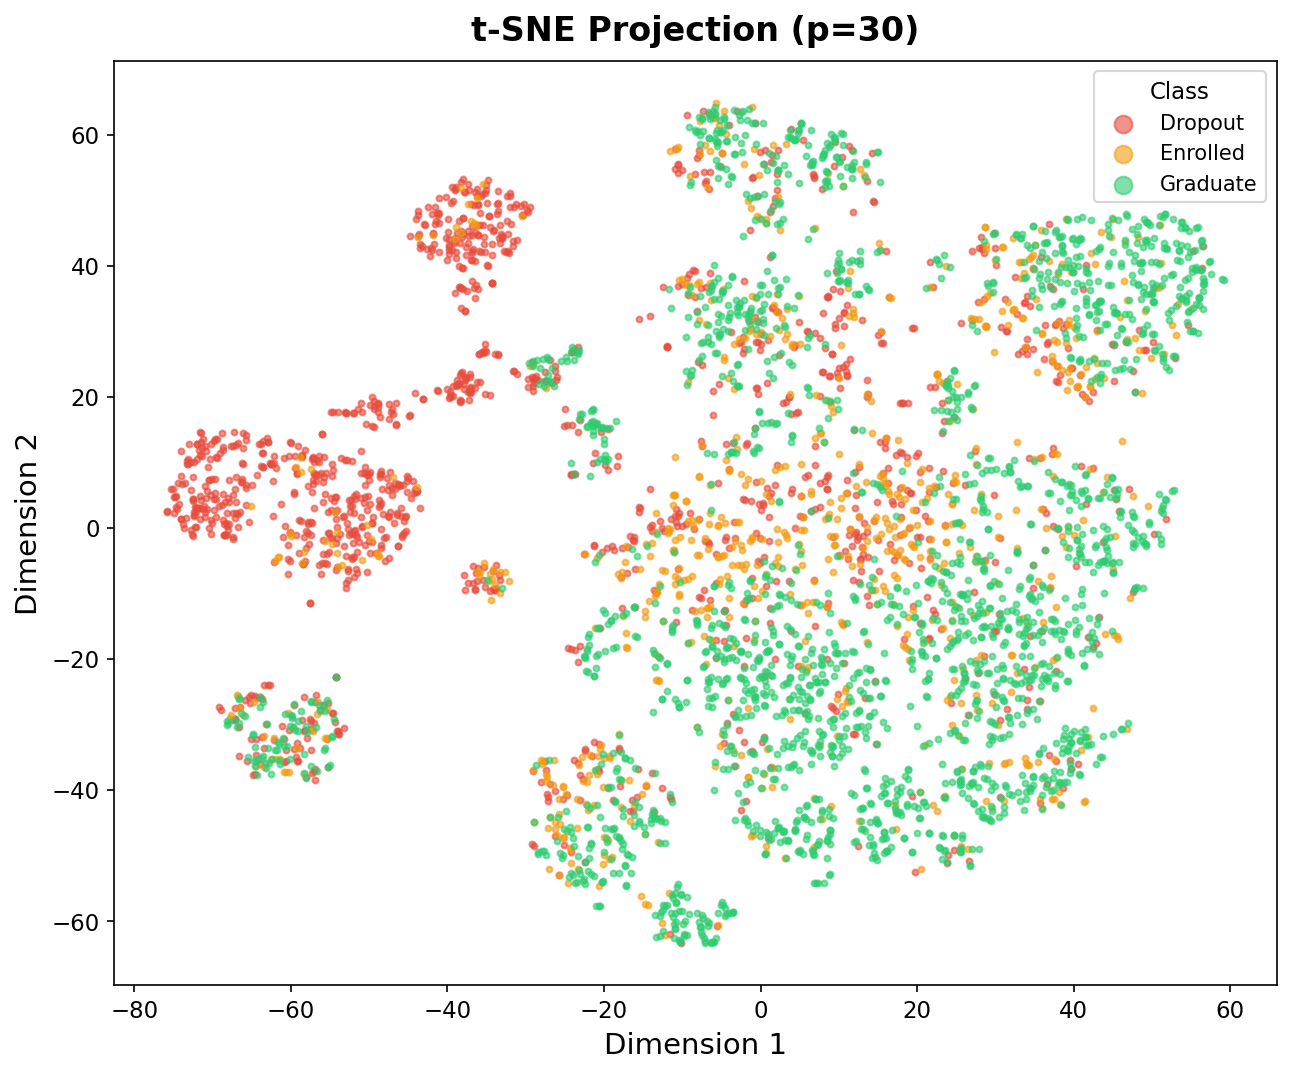
\includegraphics[width=\textwidth, height=0.45\textheight, keepaspectratio]{../data/plots/02_tsne_2d_perplexity_best.png}
    \end{column}
    
    % 图2：层次聚类
    \begin{column}{0.25\textwidth}
        \centering
        \scriptsize \textbf{Hierarchical (Ward)} \\
        \vspace{0.1cm}
        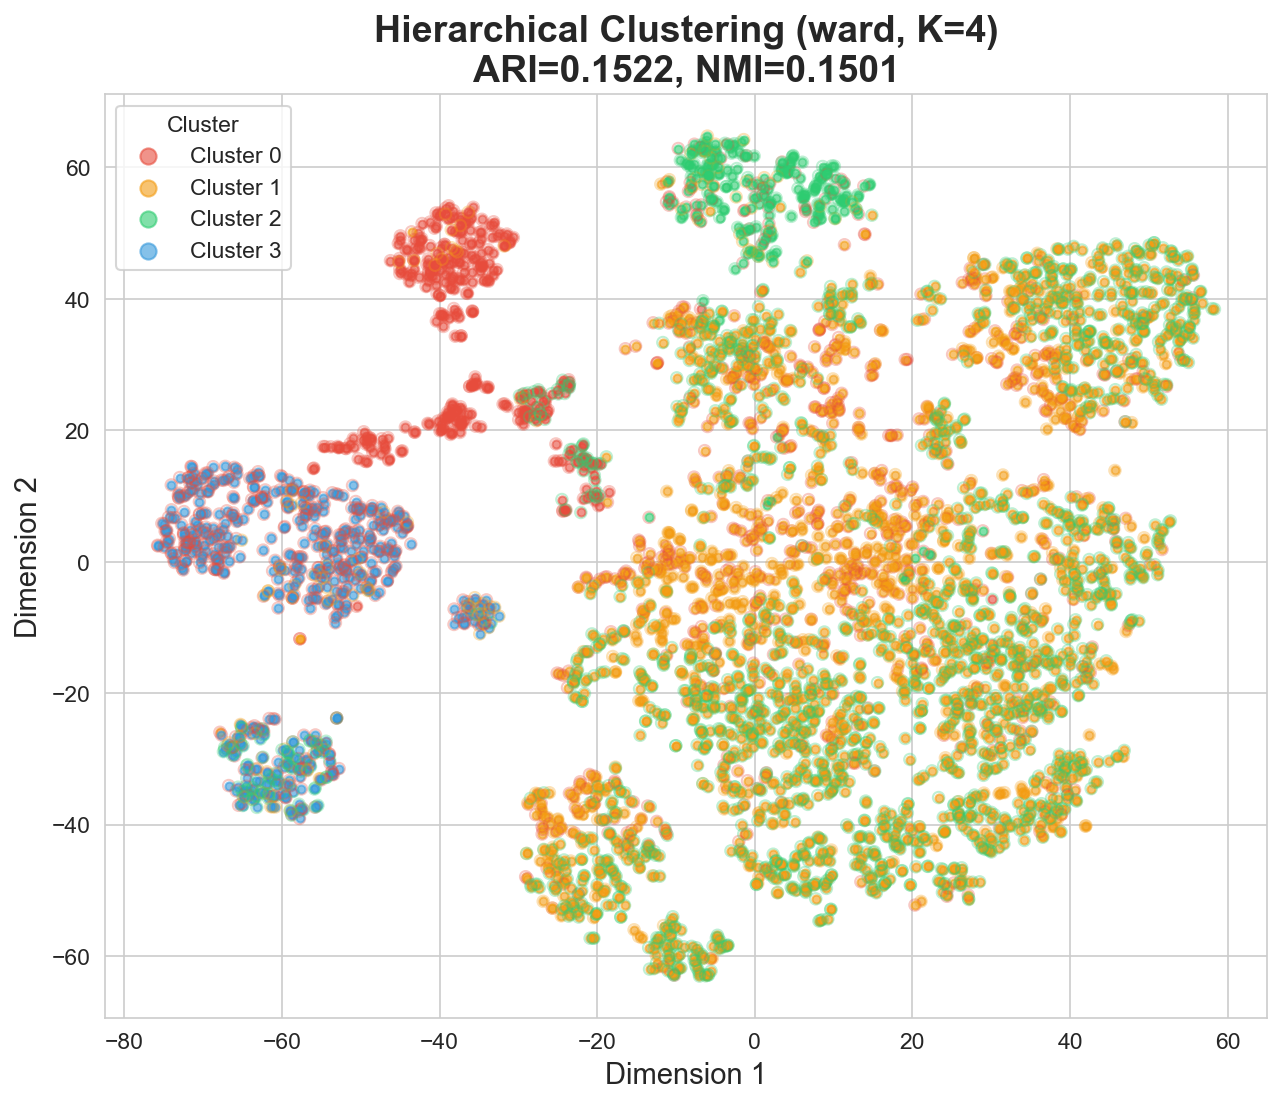
\includegraphics[width=\textwidth, height=0.45\textheight, keepaspectratio]{../data/plots/03_hierarchical_clusters_tsne.png} 
    \end{column}
    
    % 图3：K-Means
    \begin{column}{0.25\textwidth}
        \centering
        \scriptsize \textbf{K-Means ($K=4$)} \\
        \vspace{0.1cm}
        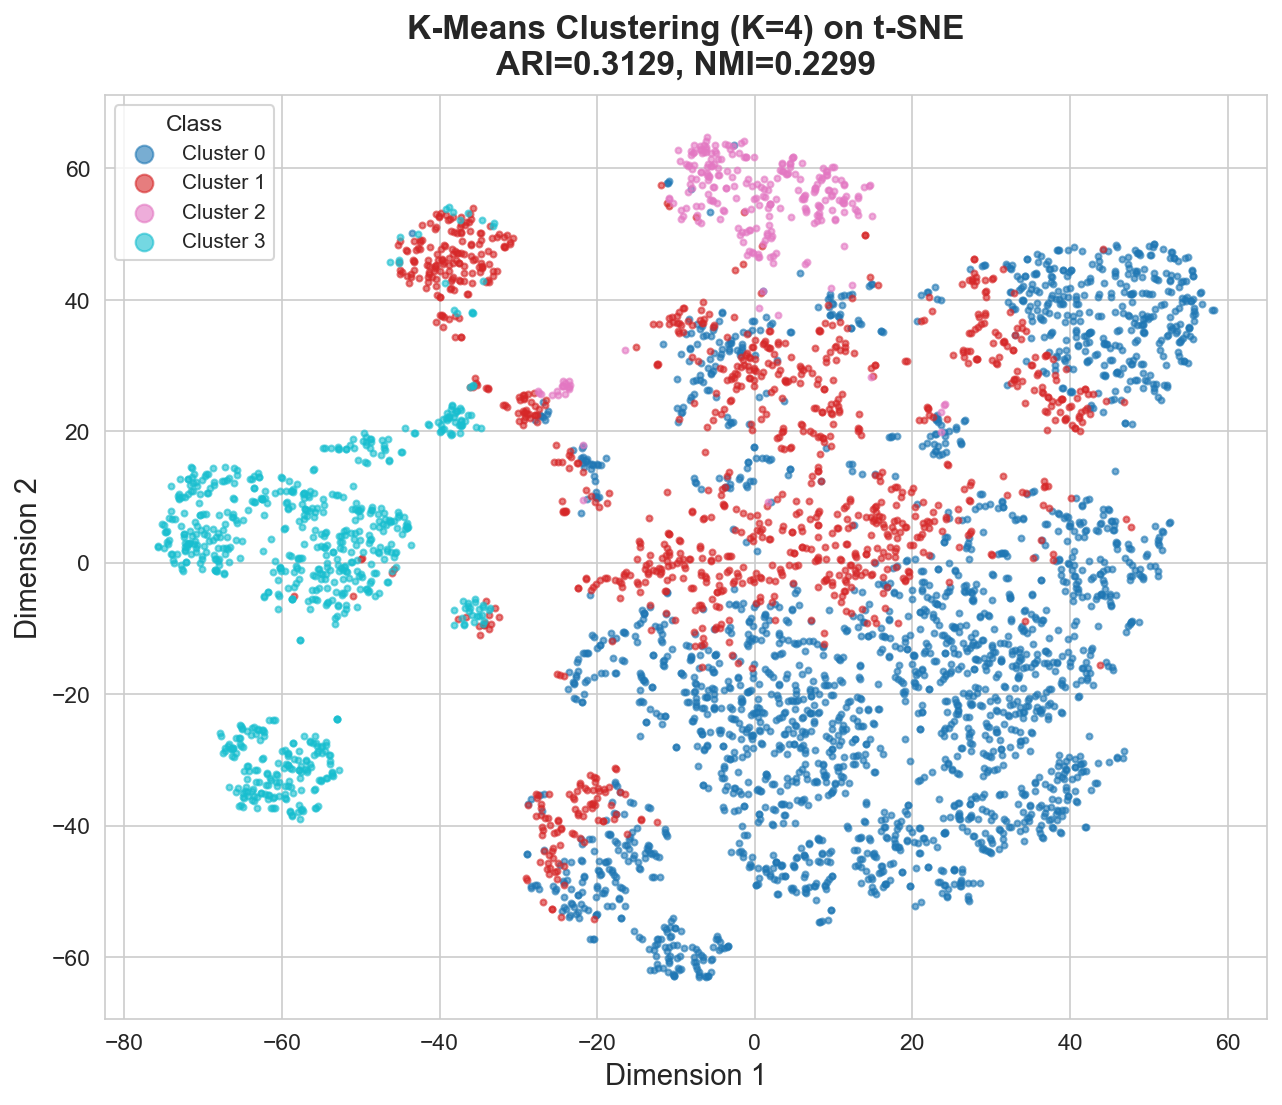
\includegraphics[width=\textwidth, height=0.45\textheight, keepaspectratio]{../data/plots/03_kmeans_clusters_tsne.png} 
    \end{column}

    % 图4：GMM
    \begin{column}{0.25\textwidth}
        \centering
        \scriptsize \textbf{GMM (Tied)} \\
        \vspace{0.1cm}
        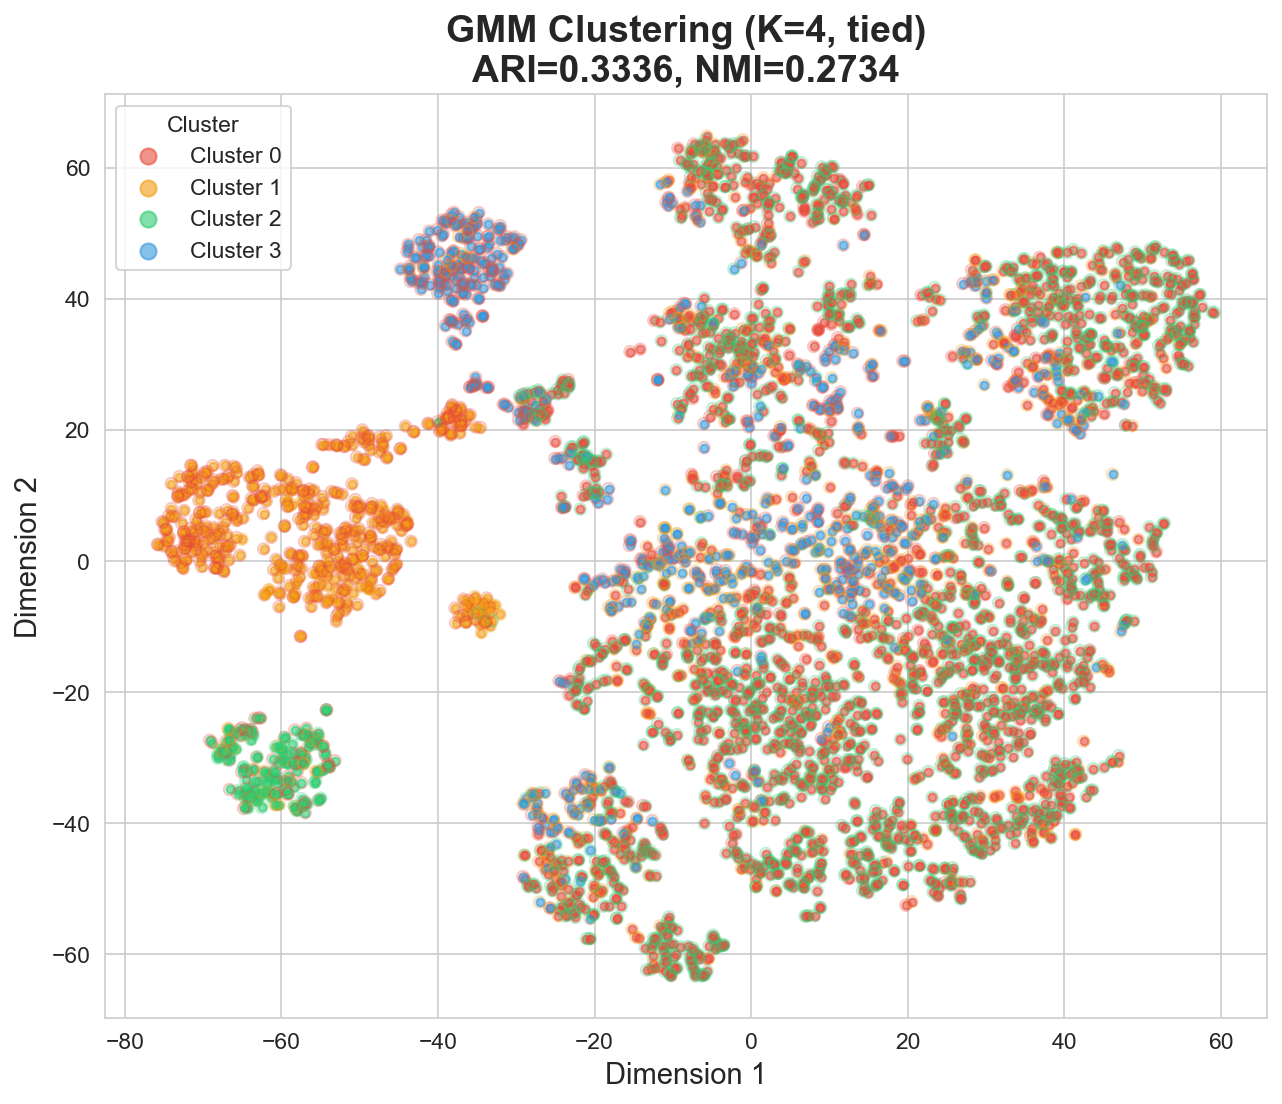
\includegraphics[width=\textwidth, height=0.45\textheight, keepaspectratio]{../data/plots/03_gmm_clusters_tsne.png} 
    \end{column}

\end{columns}

\end{frame}

\section{Part C}
\begin{frame}
\frametitle{Part C}
\end{frame}

\begin{frame}
\frametitle{Conclusion}

\textbf{Key Findings}
\begin{enumerate}
    \item Engineered top-40 features carry strong signal; academic metrics dominate.
    \item \textcolor{orange}{Enrolled} is structurally intermediate — not a natural cluster.
    \item LR is the strongest baseline; LR + class-bias tuning achieves best F1 = \textbf{0.723}.
\end{enumerate}

\vspace{0.3cm}
\textbf{Limitations \& Future Work}
\begin{itemize}
    \item LR+bias gain is borderline significant ($p = 0.051$)
    \item Future: better Enrolled modeling, external validation, early-warning deployment
\end{itemize}

\end{frame}

\section{Reference}
\begin{frame}{Reference}
\begin{thebibliography}{4}
\setbeamertemplate{bibliography item}{} 

\bibitem{realinho2022}
Realhino, V., et al. (2022).  Student Dropout and Academic Success.  UCI Machine Learning Repository. 
https://doi.org/10.24432/C5MC89


\end{thebibliography}
\end{frame}

\begin{frame}
\centering
\vspace{1cm}
{\Huge \textcolor{mainblue}{\textbf{Q \& A}}}
\vspace{1.5cm}

{\Large \textbf{Thank You!}}
\vspace{0.8cm}
\end{frame}

\end{document}
